% !TEX root = ../main.tex

% ---------------------------------------------------------------
% Background
% ---------------------------------------------------------------

\chapter{Background}\label{chap3:background}
\section{Freezing Of Gait}
Tra i sintomi della malattia di Parkinson, il Freezing può sicuramente essere considerato uno dei più debilitanti. Il Freezing nella malattia di Parkinson, detto anche acinesia paradossa, congelamento o semplicemente blocco motorio, è un’improvvisa, temporanea e involontaria incapacità di iniziare un movimento. È un disturbo che insorge nel corso dell’evoluzione della malattia di cui costituisce un sintomo indipendente e generalmente resistente al trattamento con levodopa. Tale fenomeno si può verificare in ogni momento e i pazienti che lo sperimentano affermano che: \textit{«è come se i piedi rimanessero, per qualche istante, incollati al suolo con la conseguente impossibilità di eseguire il passo successivo»}. In realtà, il Freezing si può verificare anche durante azioni differenti dal cammino come ad esempio l’alzarsi da una sedia o il raccogliere un oggetto. Alcune persone sono più predisposte di altre a subire episodi di congelamento. Tali episodi, si possono verificare sia quando il soggetto è in astinenza da farmaci dopaminergici, in questo caso si parla di “Freezing off”, sia quando il soggetto sta assumendo i farmaci, “Freezing on”. \\
È stato dimostrato che il fenomeno del Freezing nella malattia di Parkinson è spesso collegato alle frequenti cadute a cui i soggetti malati vanno incontro. Le cadute nel Parkinson si verificano più spesso quando il soggetto si gira o cambia direzione e sono frequentemente legate a diversi episodi di Freezing. Non tutti i malati di Parkinson subiscono il fenomeno del Freezing, ma si pensa che coloro che lo provano abbiano una più alta probabilità di cadere a terra. L’imprevedibilità del Freezing, accompagnata dallo sforzo inutile a cui il soggetto si sottopone per cercare di muoversi in avanti, possono causare perdita di equilibrio e quindi cadute. \\
Nel tentativo di superare questo stato di forzata immobilità, i pazienti, talora con un aiuto esterno, cercano di mettere in atto adeguate strategie che si avvalgono di stimoli sensoriali di diversa natura (tattili, visivi oppure uditivi e verbali). Alcune tecniche di tipo motorio o sensoriale possono aiutare i pazienti a convivere con il problema del Freezing. Ad esempio, un paziente incapace di iniziare il primo passo potrebbe riuscire a superare il blocco motorio adottando una delle seguenti strategie:
\begin{itemize}
	\item fare un passo in direzione di un bersaglio;
	\item fare un passo per superare un bastone posto sul pavimento;
	\item fare il primo passo marciando come un soldato.
\end{itemize}
L’idea che sta alla base di tali stratagemmi è mettere in atto un programma motorio volontario che sostituisca il programma motorio automatico malfunzionante nei malati di malattia di Parkinson. Episodi frequenti di Freezing possono avere pericolose conseguenze sia sullo stato fisico sia su quello psicologico del malato e compromettono ampiamente la qualità della vita di chi ne soffre privandolo spesso dalla propria indipendenza.\\
\subsection{Le tipologie di Fog}
Il FoG è un episodio transitorio che usualmente dura pochi secondi e di cui ancora non si conosce la patofisiologia, ossia la causa scatenante, ma è stato dimostrato che esistono più sottotipi di Freezing, che si differenziano per l'evento scatenante il fenomeno:
\begin{itemize}
	\item necessità del paziente di girare su sè stesso per cambiare direzione (esitazione legata alla svolta);
	\item attraversamento di spazi stretti, come una porta od un corridoio;
	\item inizio del movimento di camminata;
	\item regolazione dei passi in prossimità della destinazione (come ad esempio una sedia su cui sedersi);
	\item stress, come lo squillo di un telefono o campanello o quando la porta dell'ascensore si apre.
\end{itemize}
Come la malattia progredisce, però, il FoG può apparire spontaneamente anche in uno spazio aperto, evidenziando così l’aspetto imprevedibile di questo fenomeno. Inoltre, fonti di distrazione, che possono distogliere l’attenzione del soggetto dal cammino, o il compimento contemporaneo di più azioni (dual-tasking) possono aumentare la probabilità che si verifichi un episodio di Freezing.\\
\begin{figure}[]
	\centering
	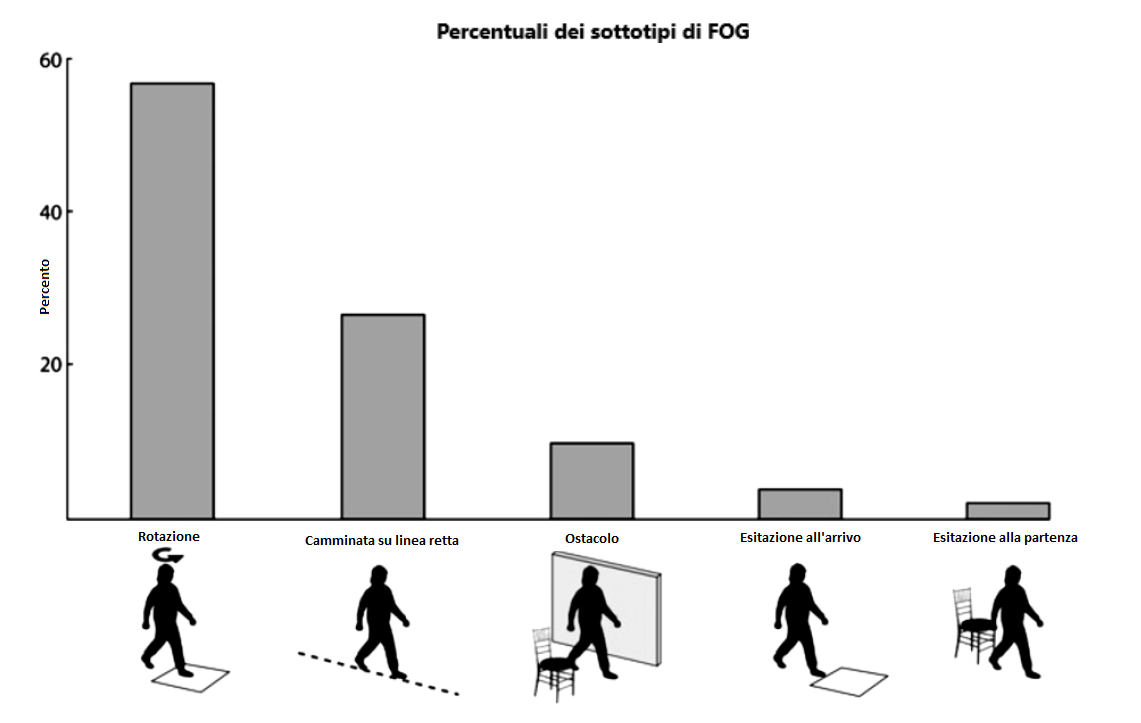
\includegraphics[scale=0.4]{images/Proportion_of_FOG_sub-types.png}
	\caption{Diversi tipi di Freezing esistenti e loro percentuale di incidenza su un certo gruppo di malati di Parkinson. [Fonte: J.M. Shine et al., 2012]}
\end{figure}
Dallo studio di Schaafsma et al.\cite{30} emerge che gli episodi di Freezing possono anche essere suddivisi in ulteriori tre sottotipi andando ad osservare i movimenti delle gambe dei pazienti e applicando la classificazione di Thompson e Marsden (1995):
\begin{enumerate}
	\item FoG associato a passi molto piccoli e strascicati con il minimo movimento in avanti (trascinamento con piccoli passi);
	\item FoG caratterizzato da tremore alle gambe, ma nessun movimento in avanti efficace (tremito da fermo);
	\item FoG caratterizzato da acinesia completa, vale a dire, nessun movimento osservabile delle gambe.
\end{enumerate}
La necessità di dividere il FoG in sottogruppi dipende dal fatto che questi ultimi potrebbero avere origine differente e quindi essere provocati da cause separate.
\subsection{Influenza del FoG nella camminata}
Il Freezing of Gait influenza il pattern del cammino sia all’inizio della deambulazione sia a regime incrementando o diminuendo in modo evidente i valori dei parametri sopra riportati. Ad esempio, nei parkinsoniani che manifestano frequenti fenomeni di Freezing, la variabilità della durata del passo risulta maggiore e la lunghezza del passo minore rispetto alle situazioni in cui il Freezing è assente. Inoltre, la velocità e la lunghezza dei primi tre passi sono significativamente inferiori nei pazienti con malattia di Parkinson e con Freezing rispetto ai soggetti sani. Anche se il Freezing è tipicamente considerato un problema motorio, il fatto che spesso compaia quando il paziente si trova in spazi ristretti, suggerisce che la percezione dello spazio contribuisce in larga misura a scatenare il sintomo\cite{37}.Inoltre, i pazienti con Freezing hanno velocità media del cammino minore rispetto a pazienti sani e subiscono una riduzione ulteriore della velocità nel momento in cui si trovano a dover attraversare una porta o uno spazio stretto. Depressione e ansia possono comportare un carico cronico sulla salute mentale, e la depressione è associata con i cambiamenti di andatura, tra cui una maggiore variabilità passo-a-passo. Il Dual-Tasking, l’ansia e la depressione possono incrementare la variabilità del passo, la di-sincronizzazione di gamba destra e sinistra e l'asimmetria nei pazienti con Parkinson riducendo così la soglia per il FoG. \\
\begin{figure}[]
	\centering
	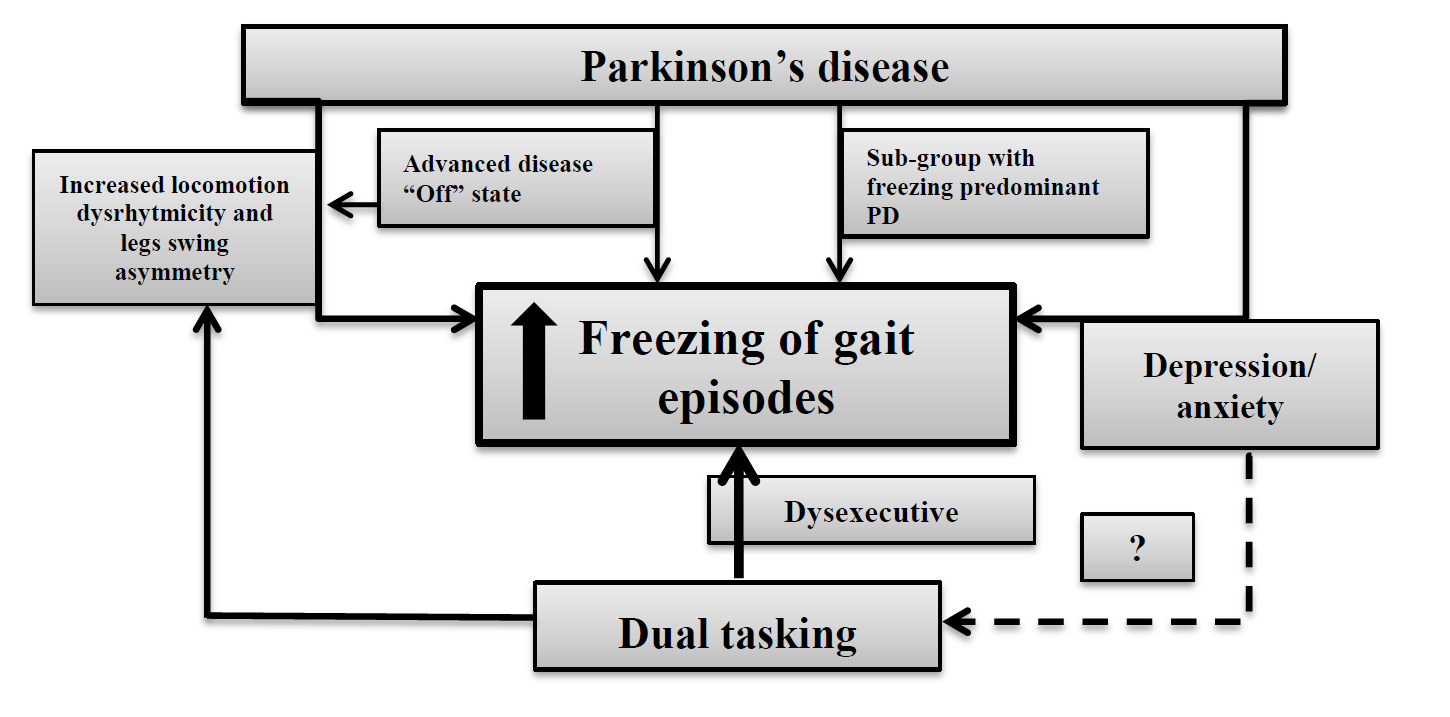
\includegraphics[scale=0.4]{images/Schema_Concettuale_Stress.png}
	\caption{Quadro concettuale relativo al Freezing of Gait (FoG) riguardante aspetti mentali e motori.}
\end{figure}

\section{Machine Learning}
Il Machine Learning si occupa della realizzazione di sistemi che si basano su osservazioni o esempi come dati per la sintesi di nuova conoscenza (classificazioni, generalizzazioni, riformulazioni). Il Machine Learning (ML) o Apprendimento automatico è una disciplina scientifica che progetta e sviluppa algoritmi che consentono agli elaboratori di evolvere il proprio comportamento basandosi su dati empirici. Il principale obiettivo di ricerca in ambito di Machine Learning è “imparare” a riconoscere automaticamente pattern complessi ed effettuare scelte intelligenti basandosi su dati già analizzati. La necessità di ricorrere al ML nasce dal fatto che prevedere a priori l'intero set di possibili comportamenti in base all'input, costruendo per esempio manualmente un set di regole, è troppo complesso da descrivere in un linguaggio di programmazione. Parallelamente, la difficoltà di tale metologia risiede nell'incertezza con cui si individua una corrispondenza tra input e output: essa si basa su un meccanismo parametrico per la generazione dei dati, di cui però non si conoscono a priori valori esatti dei parametri.\\
Caratteristica del ML è l'induzione, ossia l’estrazione di leggi generali a partire da un insieme di dati osservati. Essa si contrappone alla deduzione in cui, a partire da leggi generali, si prevede il valore di un insieme di variabili. L’induzione parte dall’osservazione per misurare un insieme di variabili e per poi effettuare previsioni su ulteriori dati. Questo processo complessivo nel quale, a partire da un insieme di osservazioni, si vuole effettuare previsioni su nuovi dati prende il nome di inferenza.\\
Gli algoritmi di apprendimento automatico sono tradizionalmente divisi in tre principali tipologie:
\begin{itemize}
	\item \textbf{Apprendimento supervisionato}: quando l'utente fornisce esempi (e controesempi) di quello che si deve apprendere. E' il problema più studiato	nel machine learning. Esso si pone l’obiettivo di prevedere, dato un
	elemento di cui si conoscono un insieme di parametri (features), il valore di un diverso parametro di output relativo all’elemento stesso;
	\item \textbf{Apprendimento non supervisionato}: parte da osservazioni non preclassificate;
	\item \textbf{Apprendimento con rinforzo}: tecnica di programmazione che si basa sul 	presupposto che l'algoritmo possa ricevere stimoli dall'esterno a seconda
	delle scelte fatte.
\end{itemize}
Il problema del ML è definito a partire da un universo di elementi: ciascun elemento x è descritto dai valori assunti da un insieme di features considerate come input del problema. Ad ogni x è associato un valore y di output (o target). A partire dalla conoscenza di un insieme T di elementi (denominato training set) in cui ogni elemento è descritto da una coppia ($x_i$ ,$y_i$), con $x_i$ = vettore dei valori delle d features $x_{i1}, x_{i2}, ... , x_{id}$ e $y_i$ = valore di output, si vuole derivare un modello delle relazioni sconosciute tra features e valori di output, che, dato un nuovo elemento x, consenta di predire il corrispondente valore di output y. 
\begin{figure}[]
	\centering
	\includegraphics[scale=0.8]{images/Tipologie_Machine_Learning.png}
	\caption{Schema delle tipologie di Machine Learning}
\end{figure}
Lo scopo dell'apprendimento supervisionato è di costruire un \textbf{modello di predizioni} basato su evidenze in presenza di incertezze. Un algoritmo di apprendimento supervisionato prende un insieme conosciuto di dati di input e di risposte ai dati (output) ed allena un modello al fine di generare predizioni ragionevoli a nuovi dati di input. Esistono due tecniche per questo approccio:
\begin{itemize}
	\item \textbf{Classificazione}: tecnica per predire risposte discrete, classificando i dati di input in categorie;
	\item \textbf{Regression}: tecnica per predirre risposte continue.
\end{itemize}
L'apprendimento non supervisionato, invece, trova pattern nascosti o strutture intrinseche nei dati. Tale tecnica è usata per identificare inferenze da un dataset consistente di dati di input senza classi già definite. Il clustering è l'approccio più diffuso di tale tecnica ed è utilizzato per trovare gruppi nei dati.\\
Con il ML difficilmente c'è una strada diretta dall'inizio alla fine della progettazione, ma si continua ad iterare e provare idee ed approcci differenti. Per questo è importante definire uno schema di lavoro generale ed evidenziare alcuni punti di decisione chiave lungo il percorso:
\begin{enumerate}
	\item Accesso e caricamento dei dati: questi possono essere di tutte le forme e i tipi, incompleti o mescolati;
	\item Pre-processamento dei dati: applicazione di filtri o ri-campionamento;
	\item Derivazione di feature:trovare caratteristiche peculiari a partire dai dati;
	\item Allenamento del modello di ML: può essere un procedimento lungo, poichè dipende da molti parametri;
	\item Integrazione del modello in un sistema di produzione.
\end{enumerate}
\begin{figure}[]
	\centering
	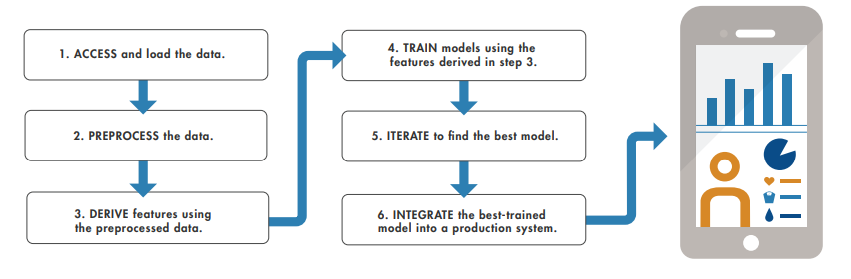
\includegraphics[scale=0.8]{images/Workflow_ML.png}
	\caption{Esempio di Workflow tramite Machine Learning}
\end{figure}
La scelta della modalità supervised o unsupervised si basa sui vantaggi e svantaggi di entrambe: la modalità supervised riesce a predire la giusta classe per le istanze appartenti al test set ma richiede una consistente quantità di istanze annotate e
questo può rappresentare un processo costoso se effettuato manualmente. La modalità unsupervised tipica del clustering, invece, ha il vantaggio di non richiedere un training già annotato (situazione particolarmente frequente quando si
ricorre al ML) ma difficilmente etichetta correttamente il cluster e ottiene una precisione più scarsa rispetto al primo metodo nell'associare le istanze ai cluster corretti. 

\subsection{Cluster Analysis}
Con il termine Cluster Analysis, o analisi dei gruppi, si intendono le procedure che permettono di individuare, all'interno di un insieme di oggetti di qualsiasi natura, alcuni sottinsiemi, \textbf{clusters} appunto, mutuamente esclusivi e tendenzialmente omogenei al loro interno. Le tecniche di Cluster Analysis creano i gruppi in modo tale che ogni osservazione sia molto simile a tutte le altre che appartengono allo stesso gruppo, in funzione di alcuni criteri prestabiliti. Alla fine del procedimento, i cluster finali dovrebbero esibire un'alta omogeneità interna (intra-cluster) ed un'alta eterogeneità esterna (inter-cluster), quindi gli oggetti all'interno dei cluster saranno vicini tra loro, mentre gli oggetti che appartengono a differenti cluster saranno più lontani tra loro.\\
La cluster analysis rientra tra le tecniche di tipo esplorativo e pertanto non è necessaria alcuna assunzione a priori, anche se impone una serie di decisioni durante l'analisi:
\begin{itemize}
	\item Scelta delle variabili;
	\item Criteri di similarità o distanza;
	\item Tecniche di aggregazione;
	\item Numero dei gruppi da ottenere;
	\item Valutazione della qualità della soluzione;
	\item Scelta fra le diverse possibili soluzioni.
\end{itemize}
\begin{figure}[]
	\centering
	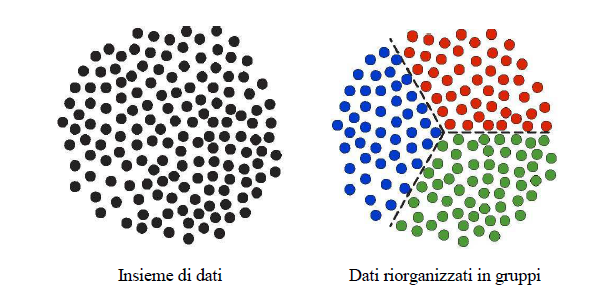
\includegraphics[scale=0.8]{images/Esempio_Cluster.png}
	\caption{Rappresentazione dei dati e dei gruppi ottenuti con la cluster analysis}
\end{figure}
Per classificare e raggruppare gli elementi in gruppi omogenei, è necessario introdurre una nozione di prossimità o similarità. Un indice di prossimità tra due generici elementi $x_i$ e $x_j$ è definito come una funzione dei rispettivi vettori riga nella matrice dei dati: $IP_{ij} = f(x_{i}^{'},x_{j}^{'}) i,j=1,2,..,n$. Due individui sono vicini quando la loro dissimilarità o distanza è piccola o, equivalentemente, quando la loro similarità è grande. Le principali misure di similarità sono illustrate in tabella \ref{TAB:SIMILARITA'}.
\begin{figure}[h!]
	\centering
	%\scriptsize
	\begin{tabular}{ l || c || c || }
		\multicolumn{1}{l||}{Tipo di dato} &  
		\multicolumn{1}{c||}{Misura} &
		\multicolumn{1}{c||}{Formula}\\
		\hline
		\hline
		Binario					&	Coefficiente di Sokal		&	$S_{ij}=(a+d)/(a+b+c+d)$	\\
		Binario					&	Coefficiente di Jaccard		& 	$S_{ij}=a/(a+b+c)$\\
		Categorici non binari	& 	Media delle variabili		&	$S_{ij}=(1/p) \sum_{k=1}^{p} s_{ijk}$\\
		Dati Continui			& 	Distanza Euclidea			&	$d_{ij}=[\sum_{k=1}^{p}(x_{ik}-x_{jk})^2]^{1/2}$\\
		Dati Continui			& 	Distanza City Block			&	$d_{ij}=\sum_{k=1}^{p}|x_{ik}-x_{jk}|$\\
		
	\end{tabular}
	\vspace{0.1cm}
	\caption{Misure di Similarità}
	%\vspace{-0.2cm}
	\label{TAB:SIMILARITA'}
\end{figure}
\\
I principali algoritmi di clustering sono:
\begin{itemize}
	\item \textbf{K-means}: l'obiettivo che l'algoritmo si prepone è di minimizzare la varianza totale intra-cluster. Ogni cluster viene identificato mediante un centroide o punto medio. L'algoritmo segue una procedura iterativa. Inizialmente crea K partizioni e assegna ad ogni partizione i punti d'ingresso o casualmente o usando alcune informazioni euristiche. Quindi calcola il centroide di ogni gruppo. Costruisce quindi una nuova partizione associando ogni punto d'ingresso al cluster il cui centroide è più vicino ad esso. Quindi vengono ricalcolati i centroidi per i nuovi cluster e così via, finché l'algoritmo non converge;
	\item \textbf{K-medoids}: è molto simile al k-means, con la sola condizione che il centroide deve corrispondere ad un elemento;
	\item \textbf{Gerarchico}: produce insiemi nidificati di clusters analizzando la similarità tra coppie di oggetti e raggruppando gli elementi in un albero binario gerarchico. Ne esistono di due tipi: agglomerativo, ossia ogni elemento è un cluster e si uniscono tra di loro fino ad arrivare ad unico cluster, e divisivo, nel quale, all'inizio, ho un unico grande cluster che poi viene diviso;
	\item \textbf{Self-Organizing Map}: sono reti neurali a connessioni laterali dove i neuroni di uscita sono organizzati in griglie di bassa dimensione (2D o 3D). Ogni ingresso è connesso a tutti i neuroni di uscita e ad ogni neurone è associato un vettore dei pesi della stessa dimensione dei vettori d'ingresso. La dimensione del vettore d'ingresso è generalmente molto più alta della dimensione della griglia di uscita;
	\item \textbf{Fuzzy C-means}: molto simile anch'esso al K-means, con la sola condizione che un elemento può appartenere a più di un cluster contemporaneamente;
	\item \textbf{Gaussian Mixture Models}: è un modello probabilistico utilizzato per modellare distribuzioni complesse di dati: l’idea base del modello è quella di suddividere un generico dataset di dati(popolation) in diverse partizioni (subpopolation) e rappresentare queste ultime attraverso una funzione di densità di probabilità. L’obiettivo è quindi rappresentare un segnale complesso attraverso una combinazione lineare di semplici distribuzioni di probabilità (Mixture Model) utilizzando, come si può intuire dal nome stesso del modello, un insieme di gaussiane per la modellazione di distribuzioni complesse di dati.
\end{itemize}
\begin{figure}[]
	\centering
	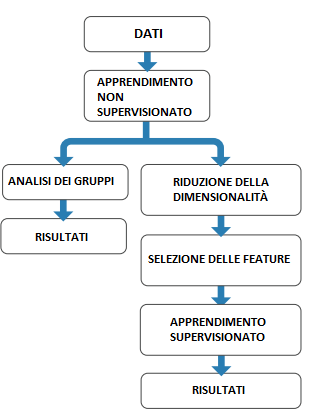
\includegraphics[scale=0.8]{images/Approcci_Clustering.png}
	\caption{Rappresentazione dei possibili approcci usando strategie di clustering}
\end{figure}
\subsection{Classificazione}
I principali approcci di classificazione sono due. In un modello parametrico, il modello stesso è preventivamente caratterizzato da un vettore X di parametri: si suppone quindi che esista una relazione tra features e input e che tale relazione sia rappresentabile all’interno di una famiglia di
relazioni parametriche rispetto a X che costituisce un modello; in altre parole, un'assegnazione di valori al vettore X definisce una specifica relazione della famiglia. Gli elementi nel training set sono utilizzati proprio per derivare tale
assegnazione di valori ai parametri (o una distribuzione di probabilità per tali valori), dopo di che non sono più utilizzati. In un modello non parametrico, invece, il numero di parametri cresce con la dimensione del training set: sostanzialmente, ogni singola previsione, in questo caso, richiede l’utilizzo dell’intero training set. Un esempio di approccio non parametrico sono i classificatori di tipo nearest neighboor, in cui si determina l'elemento $x_i$ del training set più vicino a x e si impone il valore della nuova previsione y associata a x uguale al valore $y_i$ dell’elemento $x_i$.\\
I principali algoritmi di classificazione sono:
\begin{itemize}
	\item \textbf{Decisione Tree}: si tratta di un classificatore con struttura ad albero, in cui ogni nodo può essere o foglia o nodo interno: se foglia, indica il valore della classe assegnata all'istanza; se nodo interno, specifica il test effettuato su un attributo. Per ciascun valore assunto da un attributo in un test, l'algoritmo crea un ramo ed il relativo sottoalbero. Il focus principale dell'algoritmo di crescita del decision tree è come scegliere gli attributi da testare in ciascun nodo interno dell'albero. L'obiettivo è selezionare gli attributi più utili per classificare le istanze di training
	attraverso una strategia top down, che consiste in una ricerca greedy degli
	attributi senza tornare a riconsiderare le precedenti scelte. Il criterio di split (suddivisione) con cui crea un nuovo nodo si basa sul massimo guadagno di informazione (info gain). In pratica sceglie l'attributo che riesce a dividere “meglio” le istanze appartenenti a classi diverse (detto anche criterio di massima riduzione di incertezza). Quando tutti gli elementi in un nodo hanno la medesima classe, l'algoritmo non procede con ulteriore split (criterio di stopping).
	\item \textbf{K-Nearest-Neighbors}: esso memorizza le istanza del training, poi, basandosi su un criterio di vicinanza, mette in relazione l'istanza da classificare con alcune istanze del training set presenti nello spazio delle feature.  In pratica, l'istanza è classificata “a maggioranza” in base alla
	classe più comune tra le k istanze più vicine del training. Tutto il lavoro è fatto dal classificatore in runtime. Data una nuova istanza x da classificare, il classificatore cerca i k esempi del training che sono più “simili” a x e
	guarda le loro etichette. Qualsiasi label ricorra più frequentemente tra le k label più vicine è scelta per assegnare la classe a x.
	\item \textbf{Support Vector Machine}:  l'idea principale di questo classificatore consiste nel rappresentare gli esempi del training come punti nello spazio mappati in modo tale che punti appartenenti a classi differenti siano separati dal più ampio gap possibile. I punti che mappano il test set saranno assegnati ad una categoria o all'altra in base al lato del gap su cui cadono. Più specificatamente, SVM costruisce un iperpiano ed esegue una buona separazione quando l'iperpiano ha la più ampia distanza dai punti di training più vicini di ciascuna classe. Ci sono molti iperpiani che potrebbero classificare il dato. La miglior scelta è quella di selezionare l'iperpiano che rappresenta la più ampia separazione, o margine, tra due classi, ossia l'iperpiano tale che la distanza tra esso e il punto più vicino su ciascun lato sia massima.
\end{itemize}
\section{Riduzione della dimensionalità}
\subsection{Analisi Delle Componenti Principali}
\begin{figure}[]
	\centering
	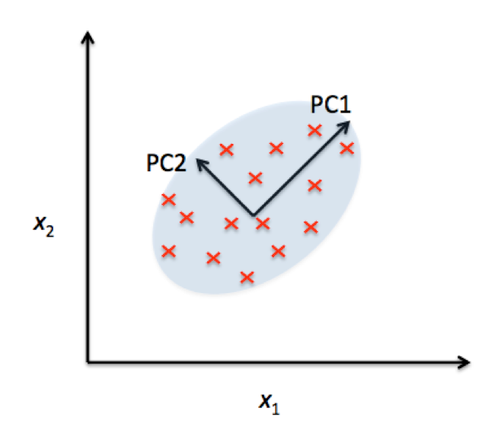
\includegraphics[scale=0.8]{images/pca.png}
	\caption{Rappresentazione del cambio di dimensionalità tramite PCA}
\end{figure}
L'analisi in componenti principali o \textbf{PCA} è una tecnica per la semplificazione dei dati, con lo scopo primario di ridurre un numero più o meno elevato di variabili in alcune caratteristiche latenti. Questo procedimento prende il nome di \textbf{feature reduction}. Ciò avviene tramite una trasformazione lineare delle variabili che proietta quelle originarie in un nuovo sistema cartesiano nel quale la nuova variabile con la maggiore varianza viene proiettata sul primo asse, la seconda variabile per dimensione della varianza sul secondo asse e così via. La riduzione della complessità avviene quindi limitandosi ad analizzare le principali (per varianza) tra le nuove variabili. Diversamente da altre trasformazioni lineari, in questa tecnica sono gli stessi dati che determinano i vettori di trasformazione.\\
Un metodo per calcolare la componente $w_i$ (ossia quella che effettua la trasformazione per la variabile i) utilizza la \textbf{matrice delle covarianze} di x, mentre un altro metodo possibile usa la matrice dei coefficienti di correlazione. Innanzitutto, si devono trovare gli autovalori della matrice di covarianza: Si ottengono così tanti autovalori quante sono le variabili x. L'autovalore con il maggiore valore corrisponde alla dimensione w che ha la maggior varianza: esso sarà dunque la varianza della componente principale numero 1. Per ciascun autovalore viene calcolato il corrispondente autovettore , ossia la matrice dei coefficienti che moltiplicano le vecchie variabili x nella combinazione lineare per l'ottenimento delle nuove variabili w. La matrice degli autovettori degli autovettori viene definita anche matrice di rotazione V e, eseguendo l'operazione $W = V*X $, dove W è il vettore colonna avente come elementi le nuove variabili $w_1,w_2,..$ e X è il vettore colonna avente come elementi le vecchie variabili $x_1,x_2,..$, si possono trovare le coordinate di ciascun punto nel nuovo spazio vettoriale. Alla fine, quindi, si tengono solo le componenti le quali, sommate tra di loro, esprimono una certa varianza (es. 90\% della varianza dei dati), mentre le altre vengono ignorate. In questo modo, partendo da n variabili iniziali, posso arrivare a (n-k) nuove variabili, dove k è il numero di componenti che non mi servono per raggiungere la soglia di varianza prefissata.
\subsection{Analisi dei Discriminanti Lineari}
Mentre la PCA è utile per la rappresentazione dei pattern (es. riconoscimento di immagini), l'analisi dei discriminanti lineari o \textbf{LDA} viene usata per discriminare tali pattern, ossia per trovare delle misure che mi permettano di dividere in più classi i miei dati. Entrambe vengono usate per la riduzione della dimensionalità delle variabili di input).\\
L'obiettivo della LDA è quello di trovare un vettore w, di traformazione, tale per cui classi differenti siano ben separate, mentre la diffusione di ogni classe sia ridotta il più possibile. In pratica, si tratta di trovare una soluzione al cosidetto criterio di Fisher: \begin{equation} J_F = \dfrac{w^TS_Bw}{w^TS_ww}  \end{equation}, nella quale $S_B$ ed $S_W$ sono rispettivamente la matrice di dispersione tra le classi e la matrice di dispersione all'interno della classe. Nel caso di due classi, la $S_B$ si calcola come: \begin{equation} S_B = (m_1 - m_2)(m_1 - m_2)^T \end{equation}, dove $m_1$ rappresenta la media della classe 1 e $m_2$ quella della classe 2. $S_w$, invece, si calcola come \begin{equation}S_W = \sum_{i=1}^{c} \sum_{x \in w_i}^{} (x - m_i)(x-m_i)^T\end{equation} con $m_i$ = media della classe i e c = numero di classi.\\
La soluzione del criterio di Fisher viene chiamata anche \textbf{Problema dell'Autovalore Generalizzato} e viene rappresentata da tale equazione: \begin{equation}S_Bw=\lambda S_ww\end{equation} e, se $S_w$ è invertibile, diventa \begin{equation}S_w^{-1}S_Bw=\lambda w\end{equation}, corrispondente al problema degli autovalori regolari che coinvolge $S_W^{-1}S_B$. Una volta che w viene trovato, le feature cercate vengono calcolate: \begin{equation}y = w^Tx\end{equation} le quali possono essere usate per allenare l'algoritmo di classificazione scelto e procedere alla predizione su nuovi dati.\\
Nel caso si abbiano più di 2 classi, la matrice di dispersione tra le classi, la quali misura la separazione tra le classi, diventa: \begin{equation}S_B=\sum_{i=1}^{c} n_i(m_i-m)(m_i-m)^T\end{equation} con $n_i$ = numero di campioni di training appartenenti alla classe i ed m = media di tutti i campioni di training. Ci saranno quindi C-1 autovettori, ognuno proveniente da una soluzione di (3.5), che potrebbero non essere ortogonali tra loro ma formano uno sottospazio lineare tale per cui il criterio di Fisher è massimizzato. Questi vengono inseriti in una matrice W e si calcolano le feature come in (3.6). 
\begin{figure}[]
	\centering
	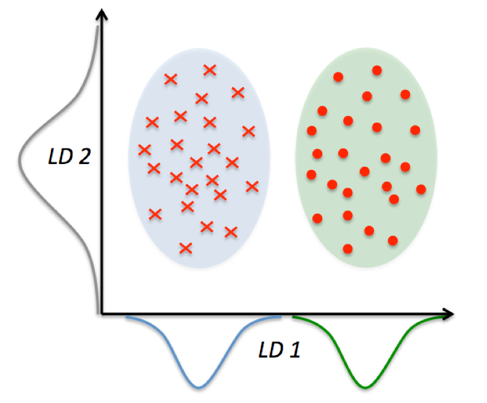
\includegraphics[scale=0.8]{images/lda.png}
	\caption{Rappresentazione del cambio di dimensionalità tramite LDA}
\end{figure}
